\documentclass[journal]{IEEEtran}

\usepackage[T1]{fontenc}
\usepackage{amsmath,amsthm}
\usepackage{newtxtext,newtxmath}
\usepackage{graphicx}
\usepackage{booktabs}
\usepackage{array}
\usepackage{multirow}
\usepackage{xcolor}
\usepackage{listings}
\usepackage{tikz}
\usetikzlibrary{arrows.meta,positioning,fit,calc,backgrounds,decorations.pathreplacing}
\usepackage{algorithm}
\usepackage{algpseudocode}
\usepackage{enumitem}
\usepackage[hidelinks]{hyperref}
\usepackage{cleveref}
\crefname{section}{Section}{Sections}
\crefname{appendix}{Appendix}{Appendices}

\setlist{nosep,leftmargin=1.2em}
\definecolor{r2blue}{HTML}{2a78d6}
\definecolor{r2orange}{HTML}{eb6834}
\definecolor{r2aqua}{HTML}{1baf7a}
\definecolor{r2gray}{HTML}{6f6e69}
\definecolor{r2light}{HTML}{eef4fc}
\definecolor{codebg}{HTML}{f7f7f5}
\lstdefinestyle{py}{
  language=Python, basicstyle=\ttfamily\scriptsize, keywordstyle=\color{r2blue}\bfseries,
  commentstyle=\color{r2gray}\itshape, stringstyle=\color{r2orange!80!black},
  backgroundcolor=\color{codebg}, frame=single, rulecolor=\color{black!12},
  numbers=left, numberstyle=\tiny\color{r2gray}, numbersep=4pt, xleftmargin=10pt,
  breaklines=true, columns=fullflexible, keepspaces=true, showstringspaces=false,
  aboveskip=4pt, belowskip=2pt}
\lstset{style=py}

\newtheorem{proposition}{Proposition}
\theoremstyle{definition}
\newtheorem{definition}{Definition}
\newtheorem{remark}{Remark}

\newcommand{\R}{\mathbb{R}}
\newcommand{\Hkv}{H_{\mathrm{kv}}}
\newcommand{\TTFT}{\mathrm{TTFT}}

\hypersetup{pdftitle={R2: A Narrow On-Device Voice Assistant with Validated Persistent Prefix KV Caching},
  pdfauthor={Siavash Shokrtalab, Alireza Panahdoost}}

\begin{document}

\title{R2: A Narrow On-Device Voice Assistant with Validated Persistent Prefix KV Caching}

\author{Siavash~Shokrtalab and Alireza~Panahdoost%
\thanks{The authors are with the Department of Computer Engineering, Islamic Azad University,
North Tehran Branch, Tehran, Iran. Code, data and benchmark scripts:
\texttt{narrow-ai-with-kv} (MIT License).}}

\maketitle

\begin{abstract}
We study a narrow design point for language-model assistants: a voice assistant for software
developers that maps each request to one of eleven typed, validated actions and runs entirely on a
laptop. The system, R2, introduces no new inference technique; it combines prefix key--value (KV)
caching, few-shot prompting, schema-constrained decoding and low-rank adaptation with a fail-closed
policy in which model output can propose but never authorise an action. Its systems contribution is
a persistent prefix cache whose reuse is conditioned on a content-derived fingerprint of the
weights, tokenizer, chat template and adapter and on a per-layer structural check, so that a stale
or damaged cache is rebuilt rather than silently reused. On an Apple M4 with Qwen3-1.7B, prefix
caching reduces time to first token from 1{,}459 to 72\,ms with unchanged outputs, and a validated
load restores readiness after a restart in 82\,ms. Against the same model on llama.cpp, warm latency
and accuracy are equal, but after a restart llama.cpp re-evaluates the prompt in 1.9\,s. On 124
author-written requests the base model is exactly right on 88.7\%, and a LoRA adapter trained on
synthetic data raises this to 96.8\% (McNemar $p=0.013$); most remaining errors stop safely rather
than act. The evaluation is limited to one machine and small, author-constructed sets.
\end{abstract}

\begin{IEEEkeywords}
KV cache, prefix caching, on-device inference, constrained decoding, tool use, voice assistants.
\end{IEEEkeywords}

% ================================================================ I
\section{Introduction}

\IEEEPARstart{L}{arge} language models (LLMs) allow more flexible voice assistants than
intent-specific pipelines, but on a laptop they introduce two costs. The first is
\emph{latency}: an instruction prompt of a thousand or more tokens must be processed before the
first output token. The second is \emph{control}: a model that can emit arbitrary text can also emit
an unintended command.

This paper describes R2, a local assistant for software developers that answers requests such as
``what is my git status?'' or ``find the Swift files''. Each request is mapped to one of eleven
intents with typed parameters, validated, confirmed by the user when it changes state, and answered
by speech. Recognition, the 1.7B-parameter language model, synthesis and all tools run on the
device.

The prompt of such a narrow assistant is dominated by a \emph{fixed prefix}---instructions, intent
catalogue and examples, 1{,}118 tokens in R2---while a request adds about 22 tokens. Reusing the KV
state of a shared prefix is standard in serving
systems~\cite{kwon2023pagedattention,zheng2024sglang,gim2024promptcache}, and saving it to storage
has been studied for multi-turn serving~\cite{gao2024cachedattention,cheng2025lmcache}. On a
single-user laptop the problem changes shape: the assistant starts and stops with the user's
session, model files and adapters change during development, and no operator notices a mismatched
cache. R2 therefore treats reuse of a stored cache as a \emph{validity} question.

The value of this work lies in the integration and its evaluation rather than in a new algorithm.
Its contributions are:
\begin{enumerate}
\item a complete on-device system that combines existing techniques under a fail-closed policy in
  which the model only proposes actions (\cref{sec:design});
\item validated cache persistence, keyed on the content of every input the cache depends on and
  checked layer by layer, with an explicit statement of the condition it enforces and of its
  residual risks (\cref{sec:validity});
\item an empirical study on Apple silicon, including a same-model comparison with llama.cpp, a cost
  model that matches measured latencies, and an ablation showing that few-shot examples provide
  most of the accuracy while caching removes their latency cost (\cref{sec:results});
\item an accuracy evaluation with exact, graded and outcome-based metrics and a parameter-efficient
  adapter trained on decontaminated synthetic data.
\end{enumerate}

% ================================================================ II
\section{Related Work}\label{sec:related}

\emph{KV caching.} Decoder-only transformers~\cite{vaswani2017attention} store the keys and values
of earlier tokens during generation; Pope et al.~\cite{pope2023efficiently} separate compute-bound
prefill from memory-bound decode. Grouped-query attention~\cite{shazeer2019fast,ainslie2023gqa}
shrinks the cache, and eviction or quantisation~\cite{xiao2024streamingllm,zhang2023h2o,
liu2024kivi,hooper2024kvquant} bounds it for long contexts.

\emph{Reusing KV state.} vLLM~\cite{kwon2023pagedattention} shares cache blocks and caches
prefixes automatically; SGLang~\cite{zheng2024sglang} keeps a radix tree of past prefixes; Prompt
Cache~\cite{gim2024promptcache} reuses prompt modules at fixed positions;
CacheBlend~\cite{yao2025cacheblend} and CacheGen~\cite{liu2024cachegen} reuse and compress
non-prefix chunks. CachedAttention~\cite{gao2024cachedattention} stores conversation KV state in
host memory and on disk between turns, and LMCache~\cite{cheng2025lmcache} adds RAM, disk and
remote tiers to serving engines. Locally, llama.cpp~\cite{gerganov2023llamacpp} and
Ollama~\cite{ollama2023} reuse the prompt prefix of a loaded model, and llama.cpp can save a slot to
a file on request; cloud APIs offer time-limited caches~\cite{anthropic2024promptcaching}.

\emph{Structured output, tools and adaptation.} Constrained decoding masks tokens that violate a
grammar~\cite{willard2023outlines,geng2023grammar,dong2025xgrammar,beurer2023lmql}; R2 uses
llguidance~\cite{llguidance2025}. Toolformer~\cite{schick2023toolformer},
ReAct~\cite{yao2023react}, Gorilla~\cite{patil2024gorilla} and BFCL~\cite{patil2025bfcl} pursue
broad tool use; R2 restricts breadth so that a small model with few-shot
prompting~\cite{brown2020language} suffices and indirect prompt injection~\cite{greshake2023injection}
cannot reach execution. LoRA~\cite{hu2022lora,aghajanyan2021intrinsic} and
QLoRA~\cite{dettmers2023qlora} adapt quantised models cheaply; MLX~\cite{hannun2023mlx},
Whisper~\cite{radford2023whisper} and Kokoro~\cite{hexgrad2024kokoro} provide the on-device stack.

\emph{Positioning.} \Cref{tab:related} compares the closest systems. Three differences matter on a
single-user laptop. (i)~\emph{Restarts:} serving engines and Prompt Cache keep reused state in a
long-running process; a laptop assistant restarts with the user's session, after updates and when
adapters change, so an in-memory cache pays the full prefill again (\cref{sec:baseline}).
(ii)~\emph{Validity:} every system in \cref{tab:related} decides reuse by matching tokens, but a KV
cache is also a function of the weights, tokenizer, template and numeric configuration. A server
guarantees these operationally; on a developer's machine a cache that matches the tokens but not
the weights yields wrong outputs without any error. (iii)~\emph{Policy:} none of these systems
governs what the generated text may cause. Reported gains are not directly comparable across
hardware---Prompt Cache reports 8--60$\times$ lower TTFT~\cite{gim2024promptcache},
CachedAttention up to 87\% lower TTFT~\cite{gao2024cachedattention}, SGLang up to 6.4$\times$
throughput~\cite{zheng2024sglang}---so we measure the local alternative directly. \Cref{app:why} lists the requirements each kind of existing tool meets.

\begin{table*}[t]
\centering\small
\caption{Prefix and KV reuse in related systems, by published design (not every configuration).
Restart: reused state survives a process restart without application code. Validity: what is
checked before reuse.}
\label{tab:related}
\footnotesize
\begin{tabular}{@{}>{\raggedright\arraybackslash}p{2.7cm}>{\raggedright\arraybackslash}p{2.7cm}>{\raggedright\arraybackslash}p{2.2cm}c>{\raggedright\arraybackslash}p{3.9cm}c>{\raggedright\arraybackslash}p{2.2cm}@{}}
\toprule
System & Reuse unit & Where stored & Restart & Validity check before reuse & Policy & Target setting \\
\midrule
vLLM APC~\cite{kwon2023pagedattention} & KV blocks & GPU memory & -- & hash of block's token prefix & -- & multi-tenant serving \\
SGLang~\cite{zheng2024sglang} & longest token prefix & GPU / host memory & -- & radix-tree token match & -- & multi-tenant serving \\
Prompt Cache~\cite{gim2024promptcache} & prompt modules & GPU / CPU memory & -- & module schema, fixed positions & -- & serving \\
CacheBlend~\cite{yao2025cacheblend} & text chunks & GPU / CPU / storage & $\circ$ & selective recompute & -- & RAG serving \\
CachedAttention~\cite{gao2024cachedattention} & conversation KV & HBM / DRAM / disk & $\circ$ & session and token match & -- & multi-turn serving \\
LMCache~\cite{cheng2025lmcache} & token chunks & RAM / disk / remote & \checkmark & chunk token hash & -- & serving engines \\
llama.cpp / Ollama~\cite{gerganov2023llamacpp,ollama2023} & prompt / slot state & RAM; file on request & $\circ$ & token match & -- & local, single user \\
Provider APIs~\cite{anthropic2024promptcaching} & marked prefixes & provider, with TTL & -- & exact prefix match & -- & cloud APIs \\
\textbf{R2 (ours)} & \textbf{fixed system prefix} & \textbf{RAM + disk (LRU)} & \checkmark & \textbf{content hash of weights, tokenizer, template, adapter, KV precision; per-layer check} & \checkmark & \textbf{single-user laptop} \\
\bottomrule
\end{tabular}
\end{table*}

% ================================================================ III
\section{System Design}\label{sec:design}

R2 maps an utterance $u$ and a short history to a decision $d=(i,\theta)$ with intent
$i\in\mathcal{I}$, $|\mathcal{I}|=11$, and parameters $\theta\in\Theta_i$, then executes,
confirms, clarifies or declines. Its objectives, in priority order, are safety, accuracy and
latency. \Cref{fig:arch} shows the components; a Python core holds inference and policy, and the
SwiftUI, terminal and notebook clients are thin. Implementation details are in \cref{app:impl}.

\begin{figure*}[t]
\centering
\resizebox{\textwidth}{!}{%
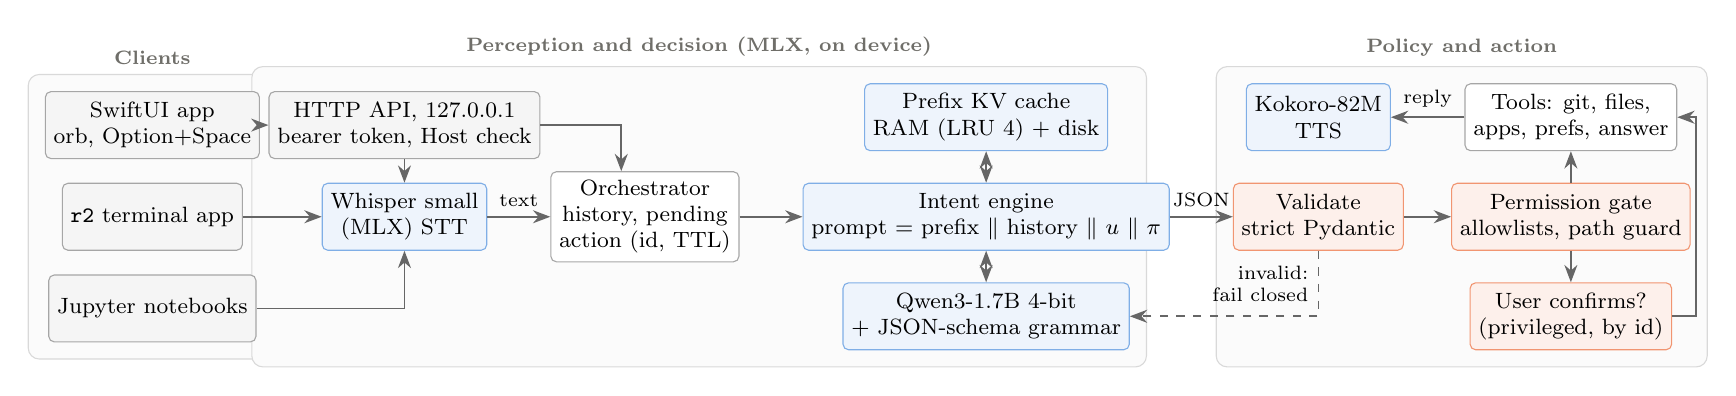
\begin{tikzpicture}[
  font=\footnotesize, >={Stealth[length=2.2mm]},
  box/.style={draw=black!35, rounded corners=2pt, fill=white, align=center, minimum height=8.5mm, inner sep=3pt},
  model/.style={box, fill=r2light, draw=r2blue!60},
  guard/.style={box, fill=r2orange!10, draw=r2orange!70},
  io/.style={box, fill=black!4},
  lane/.style={draw=black!15, rounded corners=4pt, fill=black!1.5, inner sep=6pt},
  arr/.style={->, draw=black!60, line width=0.6pt}]
  % clients
  \node[io] (app) {SwiftUI app\\ orb, Option+Space};
  \node[io, below=3mm of app] (cli) {\texttt{r2} terminal app};
  \node[io, below=3mm of cli] (nb) {Jupyter notebooks};
  % speech
  \node[model, right=10mm of cli] (stt) {Whisper small\\(MLX) STT};
  \node[io, above=3mm of stt] (http) {HTTP API, 127.0.0.1\\bearer token, Host check};
  % engine
  \node[box, right=8mm of stt] (orch) {Orchestrator\\history, pending\\action (id, TTL)};
  \node[model, right=8mm of orch] (engine) {Intent engine\\prompt $=$ prefix $\Vert$ history $\Vert$ $u$ $\Vert$ $\pi$};
  \node[model, above=4mm of engine] (kv) {Prefix KV cache\\RAM (LRU 4) + disk};
  \node[model, below=4mm of engine] (llm) {Qwen3-1.7B 4-bit\\+ JSON-schema grammar};
  % policy
  \node[guard, right=8mm of engine] (val) {Validate\\strict Pydantic};
  \node[guard, right=6mm of val] (gate) {Permission gate\\allowlists, path guard};
  \node[guard, below=4mm of gate] (conf) {User confirms?\\(privileged, by id)};
  \node[box, above=4mm of gate] (tools) {Tools: git, files,\\apps, prefs, answer};
  \node[model, above=4mm of val] (tts) {Kokoro-82M\\TTS};
  % arrows
  \draw[arr] (app) -- (http);
  \draw[arr] (http) -- (stt);
  \draw[arr] (http.east) -| ($(orch.north)+(-3mm,0)$);
  \draw[arr] (cli) -- (stt);
  \draw[arr] (nb.east) -| ($(stt.south)+(0,0)$);
  \draw[arr] (stt) -- node[above, font=\scriptsize]{text} (orch);
  \draw[arr] (orch) -- (engine);
  \draw[arr, <->] (kv) -- (engine);
  \draw[arr, <->] (engine) -- (llm);
  \draw[arr] (engine) -- node[above, font=\scriptsize]{JSON} (val);
  \draw[arr] (val) -- (gate);
  \draw[arr] (gate) -- (conf);
  \draw[arr] (gate) -- (tools);
  \draw[arr] (conf.east) -- ++(3mm,0) |- (tools.east);
  \draw[arr] (tools.west) -- node[above, font=\scriptsize]{reply} (tts.east);
  \draw[arr, dashed] (val.south) |- node[pos=0.25, left, font=\scriptsize, align=right]{invalid:\\fail closed} (llm.east);
  % lanes
  \begin{scope}[on background layer]
  \node[lane, fit=(app)(nb), label={[font=\scriptsize\bfseries, text=r2gray]above:Clients}] {};
  \node[lane, fit=(kv)(llm)(orch)(stt)(http), label={[font=\scriptsize\bfseries, text=r2gray]above:Perception and decision (MLX, on device)}] {};
  \node[lane, fit=(val)(gate)(conf)(tools)(tts), label={[font=\scriptsize\bfseries, text=r2gray]above:Policy and action}] {};
  \end{scope}
\end{tikzpicture}}
\caption{R2 architecture. Blue: learned models on MLX. Orange: deterministic policy that alone can
authorise execution. The LLM only proposes a JSON decision; invalid proposals fall back to a safe
heuristic, a clarifying question or a refusal.}
\label{fig:arch}
\end{figure*}

\emph{D1: A fixed, cached prefix.} The system prompt contains 438 tokens of instructions and 25
few-shot examples (675 tokens); with the template it forms a 1{,}118-token prefix
(\cref{fig:prompt}). History (at most three compact turns), the request and the JSON prefill follow
it, so the prefix's KV state is reused unchanged. It is kept in RAM and on disk and reused only
under the conditions of \cref{sec:validity}.

\begin{figure}[t]
\centering
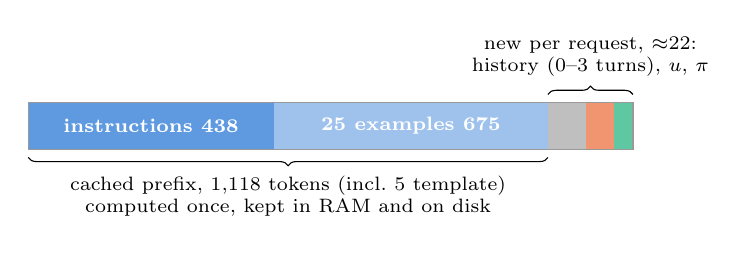
\begin{tikzpicture}[font=\scriptsize, x=0.6mm, y=1mm]
  \fill[r2blue!75] (0,0) rectangle (52,6);
  \fill[r2blue!45] (52,0) rectangle (110,6);
  \fill[black!25] (110,0) rectangle (118,6);
  \fill[r2orange!70] (118,0) rectangle (124,6);
  \fill[r2aqua!70] (124,0) rectangle (128,6);
  \draw[black!40] (0,0) rectangle (128,6);
  \node[white, font=\scriptsize\bfseries] at (26,3) {instructions 438};
  \node[white, font=\scriptsize\bfseries] at (81,3) {25 examples 675};
  \draw[decorate, decoration={brace, amplitude=3pt, mirror}] (0,-1) -- (110,-1)
     node[midway, below=3pt, align=center]{cached prefix, 1{,}118 tokens (incl.\ 5 template)\\computed once, kept in RAM and on disk};
  \draw[decorate, decoration={brace, amplitude=3pt}] (110,7) -- (128,7)
     node[midway, above=3pt, align=center]{new per request, $\approx$22:\\history (0--3 turns), $u$, $\pi$};
\end{tikzpicture}
\caption{Token layout of one request. Only the right-hand tokens (grey: history, orange: request, green: prefill $\pi$) are processed per request; after generation the cache is trimmed back to the prefix.}
\label{fig:prompt}
\end{figure}

\emph{D2: Constrain structure, not values.} Decoding is restricted to the JSON schema of a decision,
compiled from the validation models; an empty mask or matcher error permits only end-of-sequence, so
the output fails to parse and takes the closed path (proof in \cref{app:constrained}). Allow-listed
values are deliberately not constrained: when application names were an enumeration, ``open
calculator'' was decoded as \texttt{Terminal}, the nearest legal string.

\emph{D3: The model proposes, the policy decides.} Output is parsed, normalised (unknown keys are
rejected), validated, and passed to a permission gate. A decision executes only if
\begin{multline*}
\mathrm{Valid}(d)\wedge\mathrm{Allowed}(d)\wedge\mathrm{InWorkspace}(d)\\
\wedge\big(\neg\mathrm{Priv}(d)\vee\mathrm{Confirm}_{\text{user}}(d)\big),
\end{multline*}
where confirmation comes only from a later user turn and is bound to the displayed action by a
single-use identifier, a 120\,s lifetime and a digest of the decision. There is no shell tool.

\emph{D4: Bounded multi-step requests.} A request with explicit connectors becomes a plan of at most
five ordinary decisions, fixed before any tool runs and executed through the same gate; tool output
never reaches a planner, so text in a file cannot add a step.

% ================================================================ IV
\section{Analysis}\label{sec:theory}

\subsection{Prefix reuse}\label{sec:prefix}

\begin{remark}[Exact reuse; well known]\label{cor:exact}
In a causal decoder with rotary positions~\cite{su2024roformer}, the keys and values at position
$t$ depend only on $x_{1:t}$, $t$ and the parameters $\theta$. Hence a cache $C_\theta(x_{1:p})$,
extended by a suffix at positions $p+1,\dots$, gives the same logits as uncached processing, and a
cache of $x$ truncated to $\mathrm{LCP}(x,x')$ positions equals that of $x'$.
\end{remark}
\noindent This property underlies every system in \cref{tab:related}. Its preconditions---identical
parameters, tokens and positions---are what a persisted cache must preserve. They also explain two
negative results below: dropping the oldest history turn shifts all later positions, and a rotating
window shorter than the prompt removes most instructions from attention.

\subsection{Validity of a persisted cache}\label{sec:validity}

\begin{definition}
A \emph{configuration} $\kappa=(\theta,\tau,\rho,q,r,x_{1:p})$ comprises weights $\theta$ including
any adapter, tokenizer $\tau$, chat template $\rho$, KV precision $q$, runtime version $r$ and
prefix tokens $x_{1:p}$. A stored cache $\hat C$ is \emph{valid} for $\kappa$ if
$\hat C=C_\kappa(x_{1:p})$.
\end{definition}

R2 stores with each cache the fingerprint
\begin{multline}
f(\kappa)=\mathrm{trunc}_{80}\big(\mathrm{SHA\text{-}256}(\mathrm{id}(\theta),\mathrm{id}(\tau),\\
h(\rho),q,r,h(\text{prefix text}))\big),\label{eq:fp}
\end{multline}
where $\mathrm{id}$ is a content identity: the SHA-256 under which the Hugging Face cache stores a
file~\cite{hfcache2025}, read from its link target without I/O; the SHA-256 of other files up to
64\,MiB; size and modification time above. A loaded cache is accepted only if (a)~its fingerprint
equals $f(\kappa)$; (b)~it has the model's number of layers, each of the expected class; (c)~every
layer's offset and key length equal $p$; and (d)~the rendered prompt begins with exactly the cached
tokens. Otherwise the prefix is rebuilt.

\begin{proposition}[Fail-closed reuse]\label{prop:validity}
If $\mathrm{id}$ is injective on the files encountered and no two configurations share an 80-bit
fingerprint, a cache written by R2 from a completed computation under $\kappa'$ and accepted under
$\kappa$ satisfies $\kappa=\kappa'$ and is valid; by \cref{cor:exact}, outputs equal those of an
uncached run up to floating-point rounding.
\end{proposition}
\begin{proof}
Acceptance implies $f(\kappa')=f(\kappa)$, hence equal identities of weights, tokenizer and
template, equal $q$, $r$ and prefix text; (d) adds equal tokens, including merges at the boundary.
A cache written from a completed computation under $\kappa'$ equals $C_{\kappa}(x_{1:p})$; atomic
renaming excludes partially written files.
\end{proof}

The assumptions delimit the guarantee. The size-and-time identity for large files outside the model
cache is not injective. An accidental collision among $k$ stored files has probability at most
$k^2/2^{81}$. Checks (b)--(c) detect truncation and architectural mismatch deterministically, but
array contents are not checksummed, so shape-preserving corruption is not detected. Because KV state
depends on $\theta$, switching adapters rebuilds the prefix (1.5\,s); an adapter on layers 21--28
leaves layers 1--20 unchanged, so a per-layer fingerprint could share most of the cache.

\subsection{Memory and cost model}\label{sec:cost}

Each token stores keys and values per layer and KV head: $M(n)=2L\Hkv d_hb\,n$, allocated in steps
of 256 tokens. For Qwen3-1.7B ($L=28$, $\Hkv=8$, $d_h=128$, $b=2$) this is 112\,KiB per token, or
140\,MiB for R2's prefix (15\% of the 0.94\,GB of 4-bit weights). Affine $\beta$-bit quantisation
with groups of $g$ scales memory by $(\beta/8+2b/g)/b$: 0.531 at 8 bits and 0.281 at 4 bits. Under a
roofline view~\cite{williams2009roofline,pope2023efficiently},
\begin{align}
T_{\text{pre}}(N)&=a+bN+cN^2,\quad b=2P/\Pi,\ c=2LHd_h/\Pi,\label{eq:tpre}\\
T_{\text{suf}}(s\mid n)&\approx\alpha+\gamma n,\qquad T_{\text{dec}}(n)=d_0+d_1n,\label{eq:tsuf}
\end{align}
for uncached prefill of $N$ tokens, a cached $s$-token suffix and decode, with $P$ parameters per
token, $H$ query heads, throughput $\Pi$, $d_0\approx W/B$ and $d_1\approx2L\Hkv d_hb/B$ for
weight bytes $W$ and bandwidth $B$. Without overheads the speed-up is bounded by $(n+s)/s$, 51.8 for
R2, and attention matches the matrix products only at $N^\star=P/(LHd_h)$.

% ================================================================ V
\section{Experimental Setup}\label{sec:setup}

All measurements use one Apple M4 (10 CPU cores, 8-core GPU, 16\,GB unified memory, 120\,GB/s) with
\texttt{mlx-community/Qwen3-1.7B-4bit} on mlx 0.32.4 and greedy decoding. The baseline runs
\texttt{qwen3:1.7b} (Q4\_K\_M) on Ollama 0.40.13, which uses llama.cpp's Metal backend, through a
thin R2 backend that renders the prompt with the same tokenizer and template and passes R2's schema
as Ollama's \texttt{format}; parsing, validation and grading are R2's own. The two 4-bit formats
differ, so weights are not bit-identical.

All request sets were written by the authors (\cref{app:sets}): a \emph{dev} set (40) used while
designing the prompt, a \emph{fresh} set (24) written before the final prompt revision, and a
\emph{test} set (60) written later to target observed weak spots. \emph{Exact accuracy} requires the
intent and normalised parameters to match. Because exact match treats all errors alike, we add
intent macro-F1, a \emph{graded score} (0 for a wrong intent, otherwise mean per-key string
similarity, akin to partial-credit slot metrics~\cite{bastianelli2020slurp}) and an \emph{outcome}
classification of what the user experiences. Intervals are 95\% Wilson; paired comparisons use the
exact McNemar test~\cite{mcnemar1947note}.

% ================================================================ VI
\section{Results}\label{sec:results}

\subsection{Latency of prefix caching}

\begin{table}[t]
\centering\small
\caption{End-to-end cache modes, 20 requests (mean $\pm$ s.d.).}
\label{tab:kvmodes}
\setlength{\tabcolsep}{3.5pt}
\begin{tabular}{@{}lrrrr@{}}
\toprule
Mode & Setup & Prefilled & TTFT (ms) & Decision (ms) \\
\midrule
None & -- & 1{,}140 & $1459\pm38$ & $1611\pm74$ \\
Prefix (RAM) & 1.52\,s build & 22 & $\mathbf{72\pm4}$ & $227\pm46$ \\
Persistent & 82\,ms load & 22 & $\mathbf{72\pm3}$ & $229\pm45$ \\
\bottomrule
\end{tabular}
\end{table}

Prefix caching reduces end-to-end TTFT from 1{,}459 to 72\,ms (20.4$\times$) and decision latency
from 1.61 to 0.23\,s (\cref{tab:kvmodes}); greedy outputs were identical in 20/20 requests, and the
largest logit difference in bfloat16 is at most 0.5 with unchanged argmax. The persistent mode
replaces the 1.52\,s rebuild after a restart by an 82\,ms validated load.

\begin{figure*}[t]
\centering
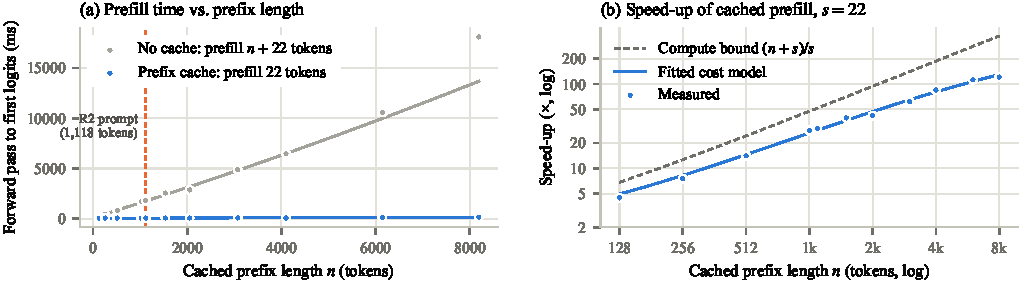
\includegraphics[width=\textwidth]{figures/scaling.pdf}
\caption{(a) Forward-pass time to the first logits for an uncached prompt of $n+22$ tokens and for
22 tokens on top of an $n$-token cached prefix; lines are the fitted models of
\cref{eq:tpre,eq:tsuf}. (b) The resulting speed-up against the compute bound $(n+s)/s$; the gap is
the fixed cost $\alpha$ of a forward pass.}
\label{fig:scaling}
\end{figure*}

Fits over 128--4{,}096 tokens (\cref{fig:scaling}) give $T_{\text{pre}}=55.4+1.460N+2.43{\times}
10^{-5}N^2$\,ms ($R^2=0.996$) and $T_{\text{suf}}=54.7+0.00621n$\,ms. The linear term implies
$\Pi\approx2.4$\,TFLOP/s, and $N^\star\approx60{,}000$ places R2 deep in the weight-bound regime.
Decoding costs $12.6+0.00149n$\,ms per token, i.e.\ 74\,GB/s effective bandwidth, at which
\cref{eq:tsuf} predicts the measured slope; every cache size matches $M$ to the byte. The model-only
speed-up at R2's length is 29.8$\times$, and end-to-end 20.4$\times$ including 11\,ms of
tokenisation and masking.

\subsection{Comparison with llama.cpp}\label{sec:baseline}

\begin{figure*}[t]
\centering
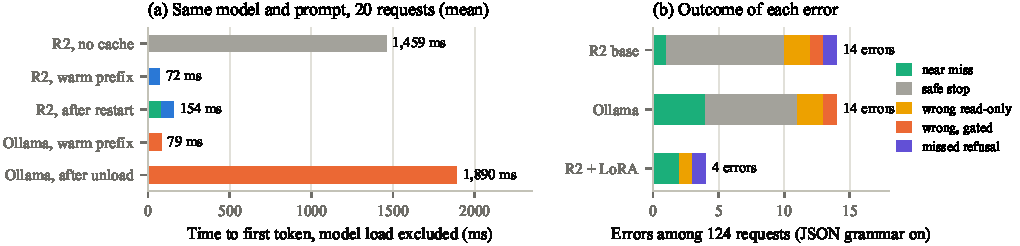
\includegraphics[width=\textwidth]{figures/comparison.pdf}
\caption{(a) Time to first token with the same model, rendered prompt and schema grammar on R2 (MLX)
and Ollama (llama.cpp), mean over 20 dev requests, model loading excluded; teal is R2's validated
cache load (82\,ms). (b) Outcome of every error among the 124 requests with the grammar: \emph{safe
stop} = clarification, refusal or help, nothing runs; \emph{near miss} = right intent, a parameter
differs; \emph{wrong, gated} = a privileged action that still needs the gate and the user.}
\label{fig:comparison}
\end{figure*}

With the same model, prompt and 20 requests (\cref{fig:comparison}a), both runtimes reuse the
prefix while the model stays loaded and reach the same TTFT (72 vs.\ 79\,ms). After the model is
unloaded---Ollama's default after five idle minutes, and the analogue of a restart---Ollama
re-evaluates the prompt in $1{,}878\pm331$\,ms, whereas R2 restores its validated prefix in 82\,ms,
23$\times$ less (model loading excluded on both sides). Outputs were identical before and after in
20/20 requests on both runtimes. Accuracy is statistically indistinguishable (\cref{tab:accuracy}):
each runtime solves six requests the other misses ($p=1.0$). On this hardware, R2's advantage over a
standard local runtime therefore lies in restart cost, validity checking and policy, not in warm
latency or accuracy.

\subsection{Conversation reuse, quantised KV and windows}\label{sec:convreuse}\label{sec:kvvariants}

\begin{table}[t]
\centering\small
\caption{Multi-turn routing: 10 sessions $\times$ 10 held-out requests,
history $\le$3 turns, all five configurations interleaved per session in rotated order. Absolute
times are higher than in \cref{tab:kvmodes} because of background load during the run; compare
rows. Pref.: tokens prefilled per turn. Exact: decision vs.\ the single-turn label.}
\label{tab:convreuse}
\setlength{\tabcolsep}{2.6pt}
\begin{tabular}{@{}lrrrrr@{}}
\toprule
History / cache & TTFT & Turns 1--4 & Turns 5+ & Pref. & Exact \\
\midrule
None / prefix & 96 & 96 & 95 & 21 & 92 \\
Sliding / prefix (default) & 254 & 192 & 295 & 103 & 90 \\
Sliding / + conversation & 235 & 138 & 300 & 87 & 90 \\
Block / prefix & 208 & 181 & 227 & 82 & 87 \\
Block / + conversation & \textbf{147} & 136 & \textbf{154} & 42 & 87 \\
\bottomrule
\end{tabular}
\end{table}

\begin{table}[t]
\centering\small
\caption{KV precision at four context lengths: cached size, 22-token
cached forward, one decode step, and the last-position logits against 16-bit.}
\label{tab:kvquant}
\setlength{\tabcolsep}{2.6pt}
\begin{tabular}{@{}rrrrrrr@{}}
\toprule
$n$ & Bits & MB & Fwd (ms) & Dec (ms) & max$|\Delta z|$ & KL \\
\midrule
1{,}118 & 16 & 146.8 & 57.4 & 15.3 & -- & -- \\
 & 8 & 78.0 & 56.2 & 13.2 & 1.1 & $10^{-8}$ \\
 & 4 & 41.3 & 56.2 & 13.3 & 48.5 & 25.8 \\
4{,}096 & 16 & 469.8 & 69.2 & 18.7 & -- & -- \\
 & 8 & 249.6 & 73.5 & 19.3 & 1.0 & $<10^{-8}$ \\
 & 4 & 132.1 & 73.1 & 18.5 & 39.2 & 6.7 \\
8{,}192 & 16 & 939.5 & 87.9 & 23.1 & -- & -- \\
 & 8 & 499.1 & 92.1 & 23.4 & 1.1 & $<10^{-9}$ \\
 & 4 & 264.2 & 100.7 & 21.0 & 37.1 & 0.23 \\
\bottomrule
\end{tabular}
\end{table}

The system prefix does not cover history, so three turns of history add about 100 prefilled tokens.
Reusing the longest prefix shared with the previous turn leaves all 100 decisions unchanged
(\cref{tab:convreuse}), but with R2's sliding window it helps only while history grows, because
dropping the oldest turn shifts all positions (\cref{sec:prefix}). A block window keeps the prefix
stable and lowers TTFT by 42\%, at a cost of 3 of 100 exact decisions; reuse therefore ships
disabled. 8-bit KV halves the cache as predicted, keeps logits within 1.1 of 16-bit and preserves
the 92.2\% exact accuracy on dev and fresh, but gives no speed-up up to 8k tokens because weight
reads dominate (\cref{tab:kvquant}). 4-bit KV changes the argmax at R2's prompt length (KL 25.8) and routing collapses
to 6.2\%; rotating windows of 1{,}024--256 positions route only 25.0--9.4\% correctly
(\cref{app:extra}).

\subsection{Accuracy and outcomes}\label{sec:accuracy}

\begin{table*}[t]
\centering\small
\caption{Exact accuracy (\%) on the three sets and pooled over 124 requests, with intent macro-F1
and graded score. $p$: exact McNemar test against the base model with the same constraint.}
\label{tab:accuracy}
\begin{tabular}{@{}llrrrlrrr@{}}
\toprule
Model & Constraint & Dev (40) & Fresh (24) & Test (60) & Pooled [95\% CI] & Macro-F1 & Graded & $p$ \\
\midrule
R2 base (MLX) & none & 87.5 & 87.5 & 80.0 & 83.9 [76.4, 89.3] & 0.850 & 0.842 & -- \\
R2 base (MLX) & json & 92.5 & 91.7 & 85.0 & 88.7 [81.9, 93.2] & 0.885 & 0.891 & -- \\
Ollama (llama.cpp) & none & 90.0 & 100 & 78.3 & 86.3 [79.1, 91.3] & 0.898 & 0.874 & 0.58 \\
Ollama (llama.cpp) & json & 95.0 & 100 & 80.0 & 88.7 [81.9, 93.2] & 0.919 & 0.899 & 1.0 \\
R2 + LoRA (MLX) & none & \textbf{100} & \textbf{100} & \textbf{93.3} & \textbf{96.8} [92.0, 98.7] & 0.986 & 0.972 & 0.0004 \\
R2 + LoRA (MLX) & json & \textbf{100} & \textbf{100} & \textbf{93.3} & \textbf{96.8} [92.0, 98.7] & 0.986 & 0.972 & 0.013 \\
\bottomrule
\end{tabular}
\end{table*}

In the default configuration (\cref{tab:accuracy}) no run produced malformed output. The prompt
revision that separated \texttt{general\_help}, \texttt{answer\_question}, \texttt{clarify\_request}
and \texttt{unsupported} raised fresh-set intent accuracy from 87.5 to 95.8\%, which, since the set
predates the revision, suggests generalisation; the harder test set reaches 85.0\%. Median decision
latency is 267--303\,ms. The graded score lies within one point of exact accuracy, so nearly every
error is a wrong intent rather than a slightly wrong parameter.

The outcome classification (\cref{fig:comparison}b) shows how the system fails. Of the base
model's 14 errors, 9 are \emph{safe stops}---a clarifying question, refusal or help text, after
which nothing runs and the user rephrases. The others are one near miss (\texttt{*.yml} for
\texttt{*.yaml}), two wrong read-only actions, one missed refusal (``commit everything'' routed to
\texttt{git\_status}, which changes nothing) and one privileged proposal (\texttt{open\_app} Finder)
that the gate refuses. The dominant pattern is that vague commands (``do the thing'', ``make it
better'') are refused as if unsafe instead of clarified: the model conflates \emph{unclear} with
\emph{unsafe}. No error executed anything outside the policy. Confusion matrices and per-intent F1
are given in \cref{app:extra}.

\subsection{Ablation}\label{sec:ablation}

\begin{table}[t]
\centering\small
\caption{Few-shot examples (FS) $\times$ decode constraint under \emph{strict} validation (unknown
keys rejected). Exact accuracy in \%; fallback rate and median decision latency on the test set.}
\label{tab:ablation3}
\setlength{\tabcolsep}{3.2pt}
\begin{tabular}{@{}clrrrr@{}}
\toprule
FS & Constraint & Dev (40) & Fresh (24) & Test (60) & Fallb. / ms \\
\midrule
 & none & 65.0 & 75.0 & 46.7 & 20.0 / 404 \\
 & intent & 65.0 & 75.0 & 46.7 & 20.0 / 381 \\
 & json & 77.5 & 87.5 & 58.3 & 0.0 / 240 \\
\checkmark & none & 87.5 & 87.5 & 80.0 & 6.7 / 332 \\
\checkmark & intent & 87.5 & 87.5 & 80.0 & 6.7 / 344 \\
\checkmark & \textbf{json} & \textbf{92.5} & \textbf{91.7} & \textbf{85.0} & \textbf{0.0} / 323 \\
\bottomrule
\end{tabular}
\end{table}

The few-shot examples are the largest factor (\cref{tab:ablation3}): with free decoding they raise
exact accuracy from 65.0 to 87.5\% on dev and from 46.7 to 80.0\% on test. They occupy 675 of the
1{,}118 prefix tokens, exactly the cost the cache removes; uncached, they would add about 0.9\,s to
every request. Constraining only the intent name changes nothing, since all preventable errors are
parameter errors. The full schema grammar removes every stray parameter that strict validation would
reject, raising accuracy by about 5 points with examples and 12 without, at no measurable latency
cost. One request is 1.7--4.2 points, so differences are indicative, but the ranking is consistent
across sets.

\begin{table}[t]
\centering\small
\caption{Planners on multi-step requests (plans validated, not executed). Fresh: 30 requests
written before the and-split and question guard existed. Rej.: share of must-refuse requests
refused.}
\label{tab:multistep}
\setlength{\tabcolsep}{3pt}
\setlength{\tabcolsep}{2pt}
\begin{tabular}{@{}lrrrr@{}}
\toprule
Planner & Dev (61) & Fresh (30), 95\% CI & Rej. & p50 \\
\midrule
Clause & 75.4 & 66.7 [48.8, 80.8] & 100 & 607\,ms \\
Clause + split + guard & \textbf{93.4} & \textbf{93.3} [78.7, 98.2] & 100 & 910\,ms \\
Model (one shot) & 47.5 & 40.0 [24.6, 57.7] & 0 & 396\,ms \\
\bottomrule
\end{tabular}
\end{table}

\emph{Multi-step planning.} On 61 dev and 30 fresh multi-step requests (\cref{tab:multistep}), the
clause planner with conjunction splitting and a question guard produces the exact plan for 93.3\% of
the fresh set and refuses every request with a destructive or out-of-scope part, at about 300\,ms of
extra routing. A one-shot model planner is faster but produces well-formed, wrong plans that no
validator can detect: it silently omits the part it should refuse (``show me the diff then change
it'' becomes the diff alone).

\subsection{LoRA adapter and voice}\label{sec:lora}

Adding examples to fix the remaining errors would lengthen the prefix, so we fine-tune instead.
Full fine-tuning needs about 27\,GB, adapter layers add latency at batch size one, and
prefix-tuning~\cite{li2021prefix} competes with the cached prefix; LoRA~\cite{hu2022lora} trains on
the 4-bit base and adds 0.15\% compute. We adapt the seven projections of the last 8 of 28 layers
($r=8$, 2.49M parameters, 0.145\% of the model) on 700 template-generated examples, discarding any
with word-set Jaccard similarity $\ge0.6$ to an evaluation request, with the loss masked to the
decision (700 steps, 78 minutes on the M4). The adapter is right on every dev and fresh request and
56 of 60 test requests, fixing 12 and breaking 2 cases with the grammar ($p=0.013$;
\cref{tab:accuracy}); it removes all safe stops and makes the grammar redundant, at unchanged TTFT.
Ranks 1--8 perform alike (96.0--96.8\%), and the learned updates are effectively low-rank
(\cref{app:lora}). Because KV state depends on the weights, the adapter's hash is part of the cache
fingerprint. On the voice path, Whisper-small transcribes in a median 269\,ms and Kokoro-82M
synthesises at 0.079 real-time factor, so a spoken request is answered in well under a second.

% ================================================================ VII
\section{Discussion and Limitations}\label{sec:limits}

\emph{What narrowness buys.} A fixed prompt makes prefix reuse exact; a closed intent set makes
constrained decoding small and its guarantee meaningful; typed decisions make authorisation a
deterministic policy. Together with the ablation this suggests a design rule for on-device
assistants: place as much of the specification as possible in a stable, validated prefix and keep
the variable part short. The price is breadth: R2 knows eleven intents and declines the rest.

\emph{Author-constructed data.} All evaluation sets and all adapter training data were created by
the authors. They reflect our phrasing and our knowledge of the system's weak spots---the test set
was written to target them---so accuracies may differ, in either direction, on requests by
independent users, and the dev set, which shaped the prompt, is optimistic.

\emph{Synthetic training data.} The adapter is trained only on template-generated utterances.
Templates cover limited syntax and vocabulary, a validation loss of 0.007 shows how easily they are
fitted, and word-overlap decontamination does not remove shared phrasing patterns. The 8.1-point gain
is therefore a gain on author-written requests, not evidence of robustness to real user language;
the adapter remains optional.

\emph{Sample size, hardware and metrics.} With 40, 24 and 60 requests, one case moves accuracy by
up to 4.2 points, and interval estimates below a few hundred datapoints are
fragile~\cite{bowyer2025clt}. All timings come from one M4; the cost model predicts how they scale
but does not replace measurement. Ollama's unload approximates a restart, and the two runtimes use
different 4-bit formats. Speech was synthesised, not recorded. The graded and outcome metrics are
automatic proxies, not a user study.

\emph{Scope of the guarantees.} \Cref{prop:validity} relies on content identities, and cache
payloads are not checksummed. The API token stops browsers and other accounts but not processes
running as the same user. Free-form answers are displayed and spoken, never executed.

\emph{Future work.} Larger request sets from independent developers and public out-of-scope
corpora; hand-written adapter training data; further Apple silicon generations; a user study with
recorded speech; per-layer fingerprints and payload checksums.

% ================================================================ VIII
\section{Conclusion}

R2 shows that a small local model can serve as a responsive and controlled voice assistant when the
system is designed for a narrow task. Its techniques are established; their combination with a
persistent prefix cache that is reused only when its validity follows from content, and with a
policy in which model output never authorises an action, yields a 72\,ms response start, 82\,ms
readiness after a restart where llama.cpp needs 1.9\,s, and 88.7\% exact accuracy (96.8\% with an
adapter) with errors that predominantly stop safely. How far these results carry to independent
users and other hardware is the main open question.

\section*{Acknowledgment}
We thank the developers of MLX, mlx-lm, llama.cpp, Ollama, Qwen3, Whisper and Kokoro. Parts of the
implementation and manuscript were prepared with the help of an AI coding assistant; the authors are
responsible for all content. S.~Shokrtalab built the system, client and tooling; A.~Panahdoost led
the research questions, methodology, analysis and evaluation design.

\bibliographystyle{IEEEtran}
\bibliography{references-ieee}

% ================================================================ appendices
\appendices
\crefalias{section}{appendix}

\section{Implementation Details}\label{app:impl}

\Cref{alg:request} gives the per-request control flow; the orchestrator keeps the last three turns
as compact JSON decisions.

\begin{algorithm}[t]
\caption{Handling one request in R2}\label{alg:request}
\small
\begin{algorithmic}[1]
\Require utterance $u$ (typed, or Whisper transcript), history $h$
\Require confirmation id $c$ (empty unless the client is answering a prompt)
\If{a pending action $P$ exists}
  \If{$u\in\textsc{Yes}$} \State $P\gets$ \textsc{Take}$(P)$ \Comment{single use}
    \State \textbf{if} $P.\textsc{Check}(c)$ \textbf{then} \Return \textsc{Execute}$(P.d)$ via the gate
    \State \textbf{else} \Return ``Cancelled.'' \Comment{missing, wrong, expired, altered}
  \ElsIf{$u\in\textsc{No}$} \State drop $P$; \Return ``Cancelled.''
  \Else\ drop $P$ and handle $u$ as a new request
  \EndIf
\EndIf
\State $x \gets \mathrm{tokens}(\text{prefix}\,\Vert\,h\,\Vert\,u\,\Vert\,\pi)$
\State $(C, x_{\text{new}}) \gets \textsc{KV.acquire}(x)$ \Comment{reuse cached prefix}
\State $y \gets \textsc{Generate}(x_{\text{new}}, C, \text{mask}=A_G(\cdot), \text{greedy})$
\State \textsc{KV.release}$(C)$ \Comment{trim back to the prefix}
\State $d \gets \textsc{ParseJSON}(\pi\Vert y)$; $d\gets\textsc{Normalise}(d)$ \Comment{unknown keys: reject}
\If{$d$ invalid} \State retry once, else heuristic / clarify / unsupported \EndIf
\State $r \gets \textsc{Gate}(d)$, then the tool's precheck \Comment{allowlist, schema, path guard}
\If{$r$ denied} \Return refusal
\ElsIf{$r$ needs confirmation} \State $P\gets(d,\ \text{id},\ \text{TTL},\ \mathrm{sha256}(d))$
  \State \Return ``Open Safari? Say yes or no.'' and the id
\Else\ \Return $\textsc{Speak}(\textsc{Execute}(d))$
\EndIf
\end{algorithmic}
\end{algorithm}

\Cref{lst:kv} shows the cache logic. The fingerprint of \cref{eq:fp} also covers the snapshot
revision, adapter files, mlx and mlx-lm versions and KV bit width. Loading is followed by
\texttt{mx.eval}, since MLX loads arrays lazily. The schema grammar is compiled by llguidance with
the separators used in the examples and no free whitespace; the mask is filled on the CPU in tens of
microseconds and applied by a Metal kernel. R2 refuses to start if the grammar is configured but
llguidance is missing.

\begin{lstlisting}[caption={Acquire, release and fingerprinted persistence (abridged from \texttt{models/kv\_cache.py}).},label={lst:kv},float=t]
def fingerprint(**parts):  # revision, weights/tokenizer/config/adapter
    h = sha256(json.dumps(parts, sort_keys=True).encode())  # shas, template,
    return {**parts, "fingerprint": h.hexdigest()[:20]}     # mlx versions, prefix

def acquire(self, full_tokens):
    n = len(self._prefix_tokens)
    if (self._cache is None or len(full_tokens) <= n
            or full_tokens[:n] != self._prefix_tokens):
        return None, full_tokens, 0          # miss: full prefill
    return self._cache, full_tokens[n:], n   # hit: suffix only

def release(self, cache):                    # keep only the prefix
    extra = cache[0].offset - len(self._prefix_tokens)
    if extra > 0:
        trim_prompt_cache(cache, extra)

def _try_load(self, fp):
    cache, meta = load_prompt_cache(path, return_metadata=True)
    mx.eval([c.state for c in cache])        # loads are lazy
    if meta.get("fingerprint") != fp["fingerprint"]:
        return False                          # stale: rebuild
    return validate_layers(cache, self._layer_classes,
                           len(self._prefix_tokens)) is None

def _save(self, fp):                          # atomic, then evict LRU
    save_prompt_cache(tmp, self._cache, metadata=fp)
    os.replace(tmp, path)
\end{lstlisting}

\emph{File tools and API.} \texttt{read\_file} opens with \texttt{O\_NOFOLLOW}, refuses non-regular
files and re-checks the real path of the opened descriptor against the workspace and secret-file
rules (\texttt{.env*}, \texttt{*.pem}, \texttt{*.key}, \texttt{.netrc}); \texttt{search\_files}
does not follow directory links and sanitises names. The loopback HTTP API, following guidance for
local MCP servers~\cite{mcpsecurity2025}, requires a loopback \texttt{Host}, refuses
\texttt{Origin} and cross-site requests, accepts only JSON or WAV bodies, and requires a bearer token
rotated on every start and stored in a \texttt{0600} file. The SwiftUI client attaches the
confirmation identifier to both the Confirm button and the next spoken ``yes''.

\section{Requirements of Existing Approaches}\label{app:why}

\Cref{tab:why} summarises which requirements typical configurations of existing tools meet for a developer who wants to query their laptop by voice. OS assistants are fast and safe but have a fixed, vendor-defined catalogue; cloud agents know developer workflows but send workspace content off the device and often expose broad tools; local chat runtimes keep data local but have no notion of a validated action; serving engines solve latency for many users but keep their cache in a long-running process and have no execution policy.

\begin{table}[t]
\centering\small
\caption{Requirements met by typical configurations of each approach (\checkmark{} yes,
$\circ$ partly or depends on configuration, -- no). Q1 on-device and private; Q2 first token
${<}100$\,ms on a laptop; Q3 typed, validated decisions; Q4 model output never authorises an
action; Q5 developer-workspace actions; Q6 fast again after a restart.}
\label{tab:why}
\setlength{\tabcolsep}{4pt}
\begin{tabular}{@{}lcccccc@{}}
\toprule
Approach & Q1 & Q2 & Q3 & Q4 & Q5 & Q6 \\
\midrule
OS voice assistant & $\circ$ & \checkmark & \checkmark & \checkmark & -- & \checkmark \\
Cloud LLM agent & -- & $\circ$ & $\circ$ & $\circ$ & \checkmark & $\circ$ \\
Local chat runtime & \checkmark & -- & $\circ$ & -- & -- & $\circ$ \\
Serving engine & $\circ$ & \checkmark & $\circ$ & -- & -- & -- \\
\textbf{R2} & \checkmark & \checkmark & \checkmark & \checkmark & \checkmark & \checkmark \\
\bottomrule
\end{tabular}
\end{table}

\section{Constrained Decoding}\label{app:constrained}

For a target language $\mathcal{L}$ (intent names, or $\mathcal{L}(G)$ for the decision grammar),
the allowed set after text $y_{<t}$ is
$A(y_{<t})=\{v:\ y_{<t}\sigma(v)\text{ is a prefix of some }w\in\mathcal{L}\}$, and logits outside
$A$ are set to $-\infty$. If $A\neq\emptyset$ at every step and generation ends when the matcher
accepts, then $y\in\mathcal{L}$: for $\mathcal{L}(G)$, $y$ names an implemented intent and contains
no parameter outside $\Theta_i$. The proof follows from the invariant that $y_{\le t}$ remains a
prefix of a string in $\mathcal{L}$. An empty $A$ or a matcher error permits only end-of-sequence.
With greedy decoding, masking changes the output only when the unconstrained argmax would leave
$\mathcal{L}$.

\section{Additional Results}\label{app:extra}

\begin{table}[t]
\centering\small
\caption{Model configuration (Qwen3-1.7B, MLX 4-bit).}
\label{tab:model}
\begin{tabular}{@{}lr@{\hspace{1.5em}}lr@{}}
\toprule
Layers $L$ & 28 & Hidden size $d$ & 2{,}048 \\
Query heads $H$ & 16 & KV heads $\Hkv$ & 8 \\
Head dim $d_h$ & 128 & FFN size & 6{,}144 \\
Vocabulary & 151{,}936 & Weights & 4-bit, group 64 \\
Weight file & 0.94\,GB & KV / token & 112\,KiB \\
\bottomrule
\end{tabular}
\end{table}
\begin{figure*}[t]
\centering
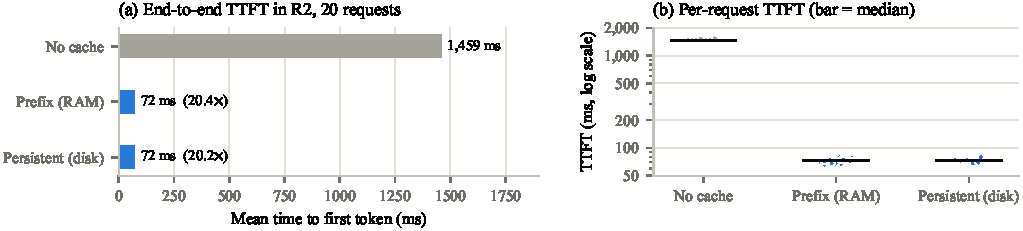
\includegraphics[width=\textwidth]{figures/kv_modes.pdf}
\caption{End-to-end TTFT inside R2 for 20 dev requests. Both cached modes reach about 71--75\,ms;
the spread across requests is small because only the short suffix varies.}
\label{fig:kvmodes}
\end{figure*}
\begin{table}[t]
\centering\small
\caption{Model-only sweep, $s=22$ (median of 5). KV is the allocated size; $\Delta z$ is the
largest absolute logit difference between cached and uncached runs.}
\label{tab:scaling}
\setlength{\tabcolsep}{3pt}
\begin{tabular}{@{}rrrrrrr@{}}
\toprule
$n$ & Uncached & Cached & $S$ & Decode & KV & $\max|\Delta z|$ \\
 & (ms) & (ms) & & (ms) & (MiB) & \\
\midrule
128 & 244 & 54.5 & 4.5 & 12.7 & 28 & 0.47 \\
256 & 428 & 56.7 & 7.6 & 12.4 & 28 & 0.38 \\
512 & 824 & 58.3 & 14.1 & 13.8 & 56 & 0.31 \\
1{,}024 & 1{,}698 & 60.3 & 28.1 & 14.4 & 112 & 0.50 \\
\textbf{1{,}118} & \textbf{1{,}813} & \textbf{60.7} & \textbf{29.8} & 12.7 & 140 & 0.44 \\
1{,}536 & 2{,}554 & 64.2 & 39.8 & 16.5 & 168 & 0.44 \\
2{,}048 & 2{,}870 & 68.0 & 42.2 & 16.3 & 224 & 0.00 \\
3{,}072 & 4{,}887 & 79.2 & 61.7 & 17.3 & 336 & 0.28 \\
4{,}096 & 6{,}478 & 76.2 & 85.0 & 18.1 & 448 & 0.00 \\
6{,}144 & 10{,}580 & 93.9 & 112.7 & 21.6 & 672 & 0.00 \\
8{,}192 & 18{,}106 & 149.6 & 121.0 & 24.9 & 896 & 0.00 \\
\bottomrule
\end{tabular}
\end{table}
\begin{figure*}[t]
\centering
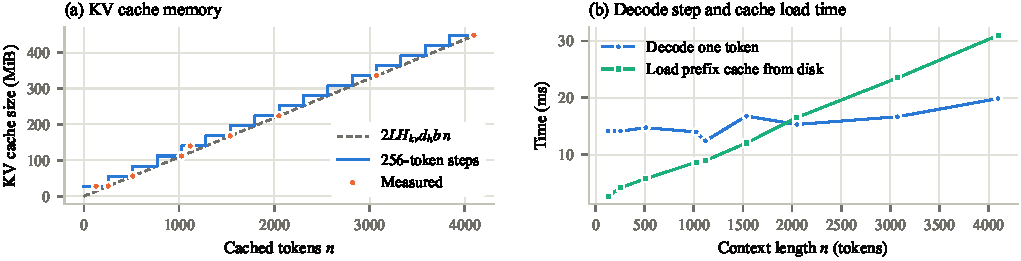
\includegraphics[width=\textwidth]{figures/memory.pdf}
\caption{(a) Measured KV size (dots) matches $M_{\text{alloc}}$ (\cref{sec:cost}) exactly, including the 256-token
allocation steps. (b) Decode time per token rises slowly with context; loading a prefix cache that
is already in the OS page cache takes 2.5--57\,ms.}
\label{fig:memory}
\end{figure*}
\begin{figure}[t]
\centering
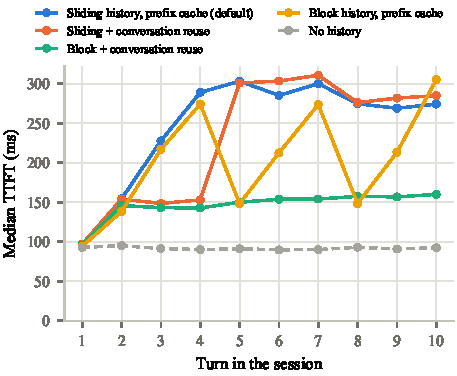
\includegraphics[width=\columnwidth]{figures/conversation.pdf}
\caption{Median TTFT by turn (10 sessions). Reuse follows the history: with a sliding window it
stops after turn 4; a block window keeps it flat.}
\label{fig:conversation}
\end{figure}
\begin{figure*}[t]
\centering
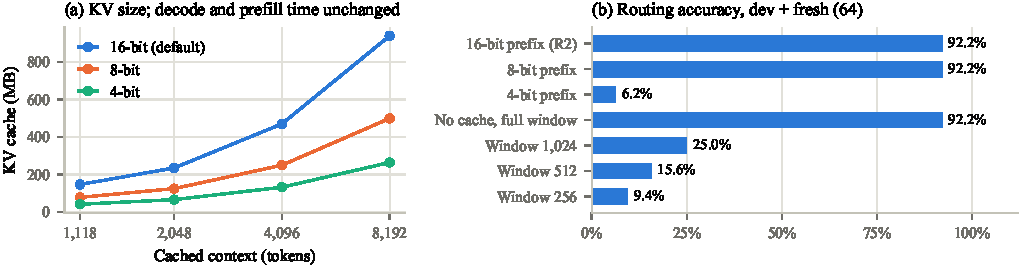
\includegraphics[width=\textwidth]{figures/kv_variants.pdf}
\caption{(a) KV size by context length and precision; it follows the ratio of \cref{sec:cost} exactly.
(b) Exact routing accuracy on dev + fresh (64 requests) for quantised prefix caches and for
rotating windows shorter than R2's 1.1k-token prompt.}
\label{fig:kvvariants}
\end{figure*}
\begin{figure}[t]
\centering
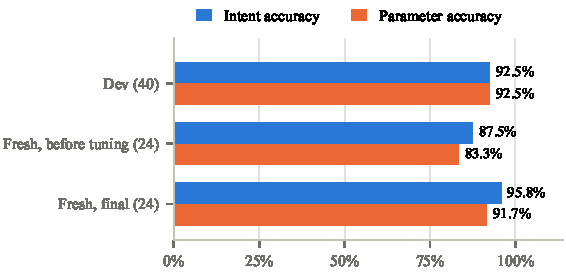
\includegraphics[width=\columnwidth]{figures/accuracy.pdf}
\caption{Intent and parameter accuracy on the dev set, on the fresh set before and after the final
prompt revision, and on the test set written later (default configuration).}
\label{fig:accuracy}
\end{figure}
\begin{figure}[t]
\centering
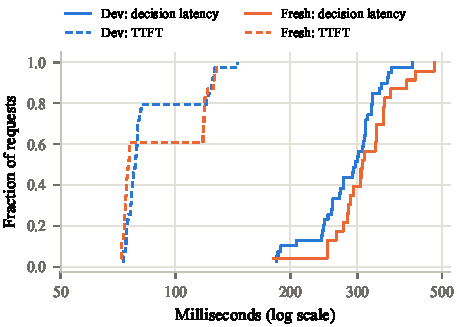
\includegraphics[width=\columnwidth]{figures/latency.pdf}
\caption{Cumulative distribution of TTFT and decision latency over the dev, fresh and test sets (the
first request, which includes GPU kernel compilation, is excluded).}
\label{fig:latency}
\end{figure}
\begin{figure}[t]
\centering
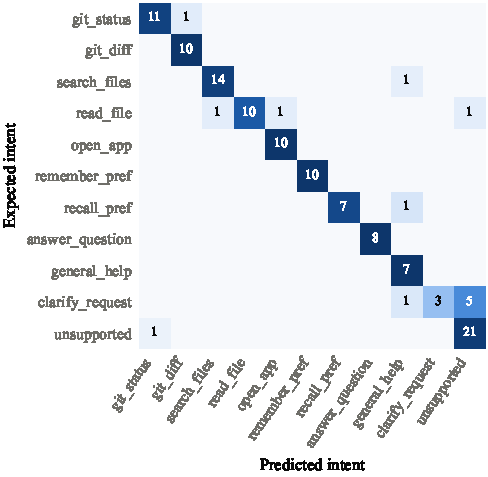
\includegraphics[width=0.92\columnwidth]{figures/confusion.pdf}
\caption{Confusion matrix over the dev, fresh and test sets (124 cases), default configuration.}
\label{fig:confusion}
\end{figure}
\begin{figure}[t]
\centering
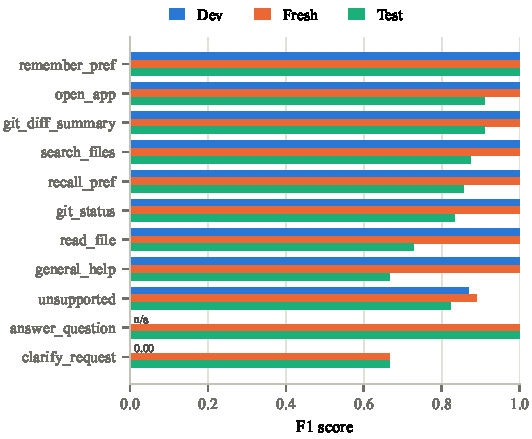
\includegraphics[width=\columnwidth]{figures/f1.pdf}
\caption{Per-intent F1 on the three sets. \texttt{answer\_question} does not occur in the dev set.}
\label{fig:f1}
\end{figure}
\begin{table}[t]
\centering\small
\caption{Exact, graded and outcome-based metrics on all 124 single-intent requests (dev, fresh and
test pooled), recomputed from the stored predictions. Outcomes: \emph{near miss} = right intent,
but a parameter differs or the decision came from the fallback; \emph{safe stop} = clarification, refusal or help instead of an action
(nothing runs); \emph{wrong read-only} = a different read-only action; \emph{wrong gated} = a
different privileged action, which still needs the gate and the user's confirmation; \emph{missed
refusal} = an out-of-scope request mapped to an action.}
\label{tab:outcomes}
\setlength{\tabcolsep}{3pt}
\begin{tabular}{@{}lrrrr@{}}
\toprule
 & \multicolumn{2}{c}{Base} & \multicolumn{2}{c}{LoRA} \\
\cmidrule(lr){2-3}\cmidrule(lr){4-5}
 & none & json & none & json \\
\midrule
Exact accuracy (\%) & 83.9 & 88.7 & 96.8 & 96.8 \\
Intent accuracy (\%) & 85.5 & 89.5 & 98.4 & 98.4 \\
Intent macro-F1 & 0.850 & 0.885 & 0.986 & 0.986 \\
Graded score & 0.842 & 0.891 & 0.972 & 0.972 \\
\midrule
Correct & 104 & 110 & 120 & 120 \\
Near miss & 2 & 1 & 2 & 2 \\
Safe stop & 13 & 9 & 0 & 0 \\
Wrong read-only & 4 & 2 & 1 & 1 \\
Wrong gated & 1 & 1 & 0 & 0 \\
Missed refusal & 0 & 1 & 1 & 1 \\
\midrule
Useful (correct + near miss, \%) & 85.5 & 89.5 & 98.4 & 98.4 \\
No unintended state change (\%) & 99.2 & 98.4 & 99.2 & 99.2 \\
\bottomrule
\end{tabular}
\end{table}
\begin{figure*}[t]
\centering
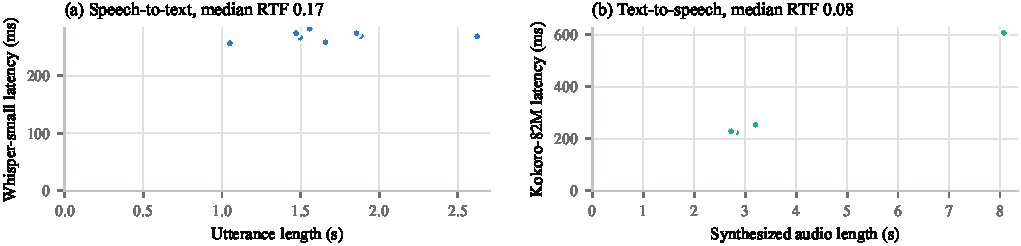
\includegraphics[width=\textwidth]{figures/voice.pdf}
\caption{On-device speech latency. (a) Whisper-small transcribes 1--2.6\,s utterances in about
0.27\,s. (b) Kokoro-82M synthesises speech about 13$\times$ faster than real time.}
\label{fig:voice}
\end{figure*}

\section{LoRA Analysis}\label{app:lora}

LoRA learns $h=W_0x+\tfrac{\alpha}{r}BAx$ with $B=0$ at initialisation; adapting matrices
$\mathcal{M}$ in $L_a$ layers trains $L_ar\sum_m(d_m+k_m)$ parameters, $8\cdot8\cdot38{,}912=2.49$M
here, exactly as reported by the trainer. With $r\in\{1,4,8,64\}$ (\cref{fig:lorarank}a), accuracy is
96.0, 96.8, 96.8 and 85.5\%; the $r=64$ result is confounded by mlx-lm's fixed $\alpha/r$. The top 8
singular directions of the $r=64$ update carry 70--87\% of $\|\Delta W\|_F^2$, against 18\% for a
random product. With $\phi(i,j)=\|U_1^{i\top}U_2^j\|_F^2/\min(i,j)$ (\cref{fig:lorasubspace}),
the row spaces of $A$ agree no better than chance, because $A$ remains near its random
initialisation, while the output directions of $\Delta W$ overlap 6--9 times the random expectation.

\begin{figure*}[t]
\centering
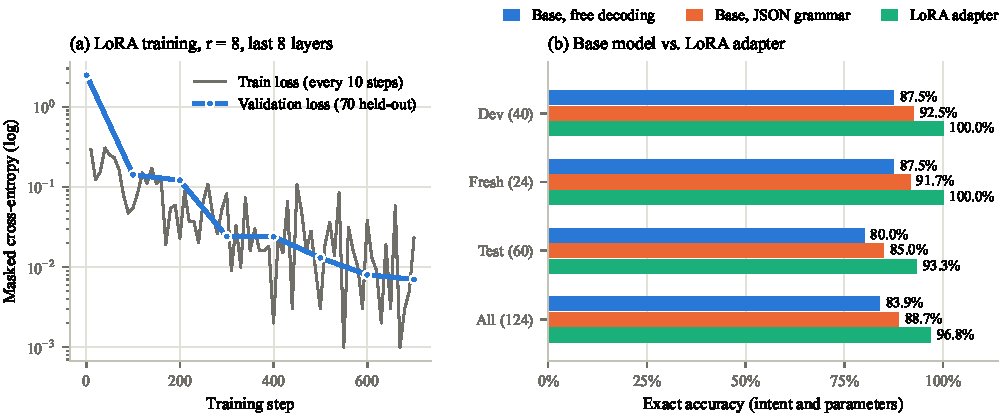
\includegraphics[width=\textwidth]{figures/lora.pdf}
\caption{(a) Loss on the decision tokens only, for training (every 10 steps) and the 70-example
validation split. (b) Exact accuracy of the base model with and without the JSON grammar and of
the LoRA adapter (grammar on; without it the adapter's numbers are identical).}
\label{fig:lora}
\end{figure*}
\begin{figure*}[t]
\centering
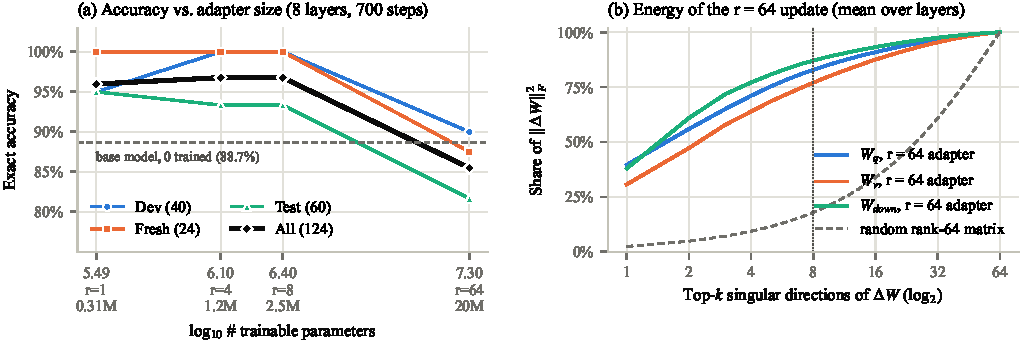
\includegraphics[width=\textwidth]{figures/lora_rank.pdf}
\caption{(a) Exact accuracy against $\log_{10}$ of the number of trainable parameters, for
LoRA ranks $r\in\{1,4,8,64\}$ on the same 8 layers, data, seed and 700 steps
(\cref{app:lora}: $311{,}296\,r$ parameters). The dashed line is the base model with few-shot
examples and the grammar. (b) Share of $\|\Delta W\|_F^2$ in the top-$k$ singular directions of
the $r=64$ updates, averaged over the 8 layers, against a random rank-64 product of the same shape.}
\label{fig:lorarank}
\end{figure*}
\begin{figure*}[t]
\centering
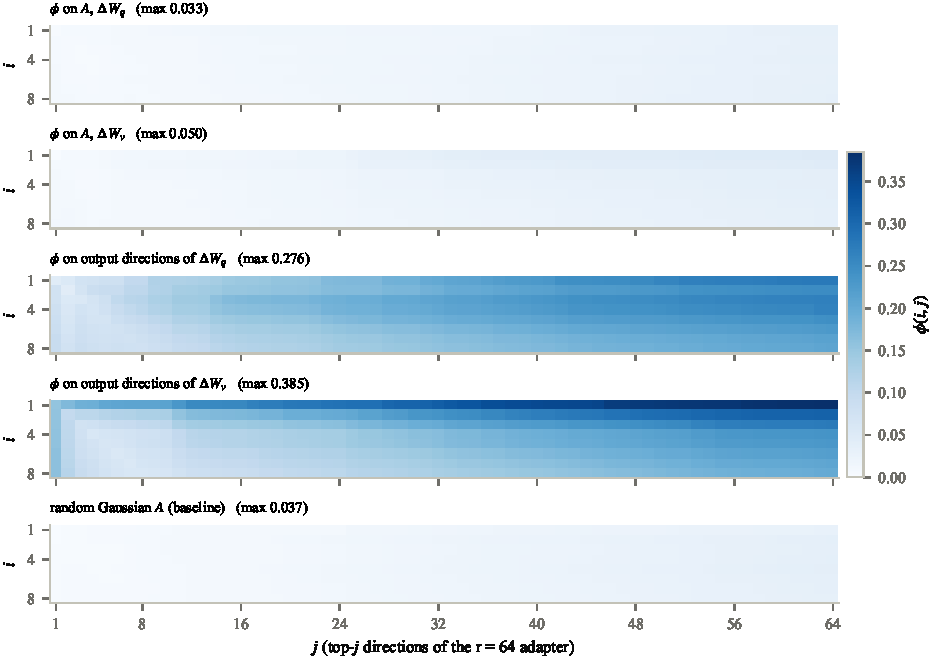
\includegraphics[width=\textwidth]{figures/lora_subspace.pdf}
\caption{Normalised subspace similarity $\phi(i,j)$ (\cref{app:lora}) between the $r=8$ and $r=64$
adapters in the last adapted layer (28), after Hu et al.~\cite{hu2022lora}. Rows 1--2: on the
row spaces of $A$, as in the original analysis; rows 3--4: on the output directions of $\Delta W$;
row 5: two random Gaussian matrices. Expected values for random subspaces are
$\max(i,j)/D$ ($D=2{,}048$ for $W_q$, $1{,}024$ for $W_v$), at most 0.03 and 0.06.}
\label{fig:lorasubspace}
\end{figure*}

\section{Prompt, Data and Reproducibility}\label{app:sets}

\subsection{System prompt excerpt}\label{app:prompt}

\begin{lstlisting}[language={},numbers=none,basicstyle=\ttfamily\scriptsize,breaklines=true]
You are R2, a narrow, local macOS developer assistant (like Siri, but only for developer tasks in the
user's active workspace).

Turn the user's request into exactly ONE JSON object and nothing else:
{"intent": "<intent>", "parameters": {...}}

Intents (parameters) - when to use:
- general_help {} - ONLY when the user asks about R2 itself: what you can do / how to use you
- git_status {} - branch, repo status, uncommitted or changed files
- git_diff_summary {} - summary or size of the diff / what changed in the code
- search_files {"pattern": "<glob, e.g. *.py, *test*, README*>"} - find, list or locate files by name or type
- read_file {"path": "<relative file path>"} - show, read, print or display the contents of a specific file
- open_app {"app_name": "<one of the approved apps>"} - launch or open an application
- remember_preference {"key": "<snake_case key>", "value": "<value>"} - user tells you a personal preference ...
- recall_preference {"key": "<snake_case key>"} - user asks about their OWN previously saved preference ...
- answer_question {"question": "<the user's question>"} - a software-development knowledge question ...
- clarify_request {"question": "<short follow-up question>"} - a vague command whose target is unclear ...
- unsupported {"reason": "<short reason>"} - chit-chat, trivia, math, destructive or out-of-scope requests
... approved apps, rules, and 25 worked examples (675 tokens) follow.
\end{lstlisting}

\subsection{Set composition}

\begin{center}\small
\begin{tabular}{@{}lrrrr@{}}
\toprule
Intent & Dev & Fresh & Test & Synthetic train \\
\midrule
\texttt{git\_status} & 4 & 2 & 6 & 53 \\
\texttt{git\_diff\_summary} & 3 & 2 & 5 & 41 \\
\texttt{search\_files} & 5 & 2 & 8 & 85 \\
\texttt{read\_file} & 4 & 2 & 7 & 91 \\
\texttt{open\_app} & 3 & 2 & 5 & 76 \\
\texttt{remember\_preference} & 3 & 2 & 5 & 61 \\
\texttt{recall\_preference} & 2 & 2 & 4 & 40 \\
\texttt{answer\_question} & 0 & 3 & 5 & 65 \\
\texttt{general\_help} & 3 & 1 & 3 & 38 \\
\texttt{clarify\_request} & 3 & 2 & 4 & 34 \\
\texttt{unsupported} & 10 & 4 & 8 & 116 \\
\midrule
\textbf{Total} & \textbf{40} & \textbf{24} & \textbf{60} & \textbf{700} \\
\bottomrule
\end{tabular}
\end{center}

All numbers are produced by scripts in the repository (\texttt{training/*.py}, including
\texttt{bench\_kv}, \texttt{bench\_scaling}, \texttt{evaluate} with \texttt{--backend mlx|ollama},
\texttt{bench\_ollama}, \texttt{ablation}, \texttt{compare\_lora} and \texttt{soft\_metrics}), stored
in \texttt{artifacts/}, and plotted by \texttt{paper/make\_figures.py}. The 255 tests run without
model downloads, a microphone or network access.

\end{document}
